%=====================================================================
%  PLANTILLA DE MEMORIA DE TRABAJO DE GRADO
%  Formato replicado de: Memoria GAMMA LAB
%  Compilar con: pdfLaTeX  (Overleaf -> Menu -> Compiler -> pdfLaTeX)
%---------------------------------------------------------------------
%  INSTRUCCIONES RAPIDAS
%  1) Suba a Overleaf las dos imagenes con estos nombres exactos:
%         imagen_logo_universidad.png
%         imagen_logo_gammalab.png
%     (tambien acepta .pdf o .jpg; si no existen se dibuja un recuadro
%      gris de reserva para que el documento compile igual)
%  2) Edite unicamente el bloque "DATOS DEL DOCUMENTO" de abajo.
%  3) Cada capitulo se crea con  \capitulo{TITULO}  (inicia pagina nueva).
%     Subcapitulos con \subsection{} y \subsubsection{} (numeracion 1.1.1).
%=====================================================================
\documentclass[12pt,letterpaper,oneside]{article}

%------------------------- Idioma y codificacion ---------------------
\usepackage[utf8]{inputenc}
\usepackage[T1]{fontenc}
\usepackage[spanish,es-noquoting,es-nodecimaldot]{babel}

%------------------------- Tipografia --------------------------------
% Fuente serif tipo Times (la del documento original).
% En Overleaf se usa newtx; si no estuviera disponible, cae en mathptmx.
\IfFileExists{newtxtext.sty}
  {\usepackage{newtxtext}\usepackage{newtxmath}}
  {\usepackage{mathptmx}}
% Alternativa: comente el bloque anterior para usar la fuente por
% defecto de LaTeX (Computer Modern).

%------------------------- Margenes y pagina -------------------------
\usepackage[
  letterpaper,
  top=2.6cm, bottom=2.5cm, left=3.0cm, right=3.0cm,
  headheight=52pt, headsep=14pt, footskip=32pt
]{geometry}

\usepackage{graphicx}
\usepackage{xcolor}
\usepackage{setspace}
\usepackage{fancyhdr}
\usepackage{titlesec}
\usepackage{ragged2e}
\usepackage[hidelinks]{hyperref}
\usepackage[normalem]{ulem}
\usepackage{soul}
\usepackage{float}

\onehalfspacing                        % interlineado 1.5
\setlength{\parindent}{1.0cm}          % sangria de primera linea
\setcounter{secnumdepth}{3}            % numera hasta 1.1.1
\setcounter{tocdepth}{3}               % indice hasta 1.1.1
\renewcommand{\contentsname}{TABLA DE CONTENIDO}

%=====================================================================
%  DATOS DEL DOCUMENTO  ->  EDITE SOLO ESTA SECCION
%=====================================================================
\newcommand{\tituloProyecto}{GAMMA LAB 2.0}
\newcommand{\tituloCorto}{GAMMA LAB 2.0}   % el que va en el encabezado
\newcommand{\grupo}{Grupo 12}

\newcommand{\autorUno}{Juan Felipe Romero Ortiz}
\newcommand{\autorDos}{Laura Juliana Garzón Arias}
\newcommand{\autorTres}{Sebastián Almanza Galvis}
\newcommand{\autorCuatro}{Xiomara Herrera Suárez}

\newcommand{\leyendaGrado}{MEMORIA DE PROYECTO DE GRADO REALIZADO PARA CUMPLIR UNO DE
LOS REQUISITOS PARA EL TÍTULO EN INGENIERÍA DE SISTEMAS}

\newcommand{\director}{Ing. Cecile Eugine Gauthier Umaña}
\newcommand{\juradoUno}{Ing. Nombre del Primer Jurado}
\newcommand{\juradoDos}{Ing. Nombre del Segundo Jurado}

\newcommand{\universidad}{PONTIFICIA UNIVERSIDAD JAVERIANA}
\newcommand{\universidadNombre}{Pontificia Universidad Javeriana} % en mayuscula/minuscula
\newcommand{\facultad}{FACULTAD DE INGENIERÍA}
\newcommand{\programa}{PROGRAMA DE INGENIERÍA DE SISTEMAS}
\newcommand{\ciudad}{BOGOTÁ, D.C.}
\newcommand{\anio}{2026}                 % año en la caratula
\newcommand{\fechaLarga}{Noviembre, 2026}      % mes y año en la portada

% Autoridades de la universidad
\newcommand{\rector}{Nombre del Rector, S.J.}
\newcommand{\decano}{Ing. Nombre del Decano de la Facultad}
\newcommand{\directorDepto}{Ing. Nombre del Director de Departamento, Ph.D.}
\newcommand{\directorCarrera}{Ing. Nombre de la Directora de Carrera}

% Nombres de los archivos de imagen (subalos con estos nombres)
\newcommand{\logoUniversidad}{imagen_logo_universidad}
\newcommand{\logoProyecto}{imagen_logo_gammalab}
%=====================================================================

%------------------- Utilidades internas -----------------------------
% Inserta la imagen si existe; si no, dibuja un recuadro de reserva.
\newcommand{\imgSegura}[3]{% {archivo}{alto}{ancho reserva}
  \IfFileExists{#1.png}{\includegraphics[height=#2]{#1.png}}{%
  \IfFileExists{#1.pdf}{\includegraphics[height=#2]{#1.pdf}}{%
  \IfFileExists{#1.jpg}{\includegraphics[height=#2]{#1.jpg}}{%
  \textcolor{gray!60}{\framebox[#3]{\rule{0pt}{#2}\scriptsize logo}}}}}}

% Texto de relleno para las secciones pendientes.
\newcommand{\pendiente}[1][Escriba aquí el contenido de esta sección.]{%
  {\color{gray!75}\itshape [#1]}\par}

% Capitulo: inicia en pagina nueva (como en el documento original).
\newcommand{\capitulo}[1]{\clearpage\section{#1}}

%------------------- Encabezado y pie de pagina ----------------------
\pagestyle{fancy}
\fancyhf{}
\fancyhead[L]{%
  \raisebox{-0.35\height}{\imgSegura{\logoUniversidad}{1.05cm}{2.2cm}}%
  \hspace{0.5cm}%
  \raisebox{-0.35\height}{\imgSegura{\logoProyecto}{0.85cm}{1.6cm}}%
}
\fancyhead[R]{\textbf{Memoria: \tituloCorto}}
\fancyfoot[R]{\textbf{Página \thepage}}
\renewcommand{\headrulewidth}{1.1pt}
\renewcommand{\footrulewidth}{1.1pt}

%------------------- Estilo de titulos -------------------------------
\titleformat{\section}
  {\normalfont\Large\bfseries}{\thesection}{0.8em}{}
\titlespacing*{\section}{0pt}{0pt}{16pt}

\titleformat{\subsection}
  {\normalfont\large\bfseries}{\thesubsection}{0.7em}{}
\titlespacing*{\subsection}{0pt}{14pt}{8pt}

\titleformat{\subsubsection}
  {\normalfont\normalsize\bfseries}{\thesubsubsection}{0.6em}{}
\titlespacing*{\subsubsection}{0pt}{12pt}{6pt}

%=====================================================================
\begin{document}

%---------------------------------------------------------------------
%  CARATULA (pagina sin numeracion). Elimine este bloque si no la usa.
%---------------------------------------------------------------------
\thispagestyle{empty}
\begin{center}
  \vspace*{1cm}
  {\large \grupo}\par\vspace{1.2cm}
  {\LARGE\bfseries \tituloProyecto}\par\vspace{2cm}
  \autorUno\par
  \autorDos\par
  \autorTres\par
  \autorCuatro\par
  \vfill
  \universidad\par
  \facultad\par
  \programa\par
  \ciudad\par
  \anio\par
  \vspace{1cm}
\end{center}
\clearpage

%---------------------------------------------------------------------
%  PAGINAS PRELIMINARES (numeracion romana: i, ii, iii, ...)
%---------------------------------------------------------------------
\pagenumbering{roman}

%------------------------ PORTADA (pagina i) -------------------------
\begin{center}
  {\Large\bfseries \tituloProyecto}\par
  \vspace{1.4cm}

  {\bfseries Autores:}\par
  \vspace{0.5cm}
  \autorUno\par
  \autorDos\par
  \autorTres\par
  \autorCuatro\par
  \vspace{1.4cm}

  \leyendaGrado\par
  \vspace{1.4cm}

  {\bfseries Director}\par
  \vspace{0.4cm}
  \director\par
  \vspace{1.2cm}

  {\bfseries Jurados del Trabajo Final de Grado}\par
  \vspace{0.4cm}
  \juradoUno\par
  \juradoDos\par
  \vspace{1.8cm}

  \universidad\par\vspace{0.6cm}
  \facultad\par\vspace{0.6cm}
  \programa\par\vspace{0.6cm}
  \ciudad\par\vspace{0.6cm}
  \fechaLarga\par
\end{center}
\clearpage

%--------------------- AUTORIDADES (pagina ii) -----------------------
\begin{center}
  {\bfseries \universidad}\par
  {\bfseries \facultad}\par
  {\bfseries \programa}\par
  \vspace{6cm}

  {\bfseries Rector de la \universidadNombre}\par
  \vspace{0.4cm}
  \rector\par
  \vspace{0.9cm}

  {\bfseries Decano de la Facultad de Ingeniería}\par
  \vspace{0.4cm}
  \decano\par
  \vspace{0.9cm}

  {\bfseries Director del Departamento de Ingeniería de Sistemas}\par
  \vspace{0.4cm}
  \directorDepto\par
  \vspace{0.9cm}

  {\bfseries Directora de Carrera de Ingeniería de Sistemas}\par
  \vspace{0.4cm}
  \directorCarrera\par
\end{center}
\clearpage

%------------------ NOTA REGLAMENTARIA (pagina iii) ------------------
\noindent{\bfseries Artículo 23 de la Resolución No. 1 de Junio de 1946}
\vspace{1cm}

\begin{justify}
\itshape
``La Universidad no se hace responsable de los conceptos emitidos por sus alumnos en sus
proyectos de grado. Sólo velará porque no se publique nada contrario al dogma y la moral
católica y porque no contengan ataques o polémicas puramente personales. Antes bien, que se
vean en ellos el anhelo de buscar la verdad y la Justicia''
\end{justify}
\clearpage

%--------------------- AGRADECIMIENTOS (pagina iv) -------------------
\section*{AGRADECIMIENTOS}
\vspace{0.6cm}

\noindent{\bfseries \autorUno:}
\vspace{0.3cm}

\pendiente[Escriba aquí los agradecimientos del primer autor. Puede usar
varios párrafos; cada uno inicia con sangría automática.]

\vspace{1cm}
\noindent{\bfseries \autorDos:}
\vspace{0.3cm}

\pendiente[Escriba aquí los agradecimientos del segundo autor.]

\vspace{1cm}
\noindent{\bfseries \autorTres:}
\vspace{0.3cm}

\pendiente[Escriba aquí los agradecimientos del tercer autor.]

\vspace{1cm}
\noindent{\bfseries \autorCuatro:}
\vspace{0.3cm}

\pendiente[Escriba aquí los agradecimientos del cuarto autor.]

\clearpage

%------------------------ TABLA DE CONTENIDO -------------------------
\tableofcontents
% Si necesita indice de figuras o tablas, descomente:
% \clearpage
% \listoffigures
% \clearpage
% \listoftables

%---------------------------------------------------------------------
%  CUERPO DEL DOCUMENTO (numeracion arabiga: 1, 2, 3, ...)
%---------------------------------------------------------------------
\clearpage
\pagenumbering{arabic}

%=====================================================================
\capitulo{INTRODUCCIÓN}
\pendiente

%=====================================================================
%=====================================================================
\capitulo{DESCRIPCIÓN GENERAL}

\subsection{Oportunidad y problema}

Las señales electroencefalográficas (EEG) son el registro de la actividad eléctrica generada por el cerebro, captada mediante electrodos. Esta actividad se puede representar mediante ondas cerebrales que se pueden estudiar en diferentes dominios de tiempo, frecuencia o tiempo-frecuencia, reflejando diferentes estados del individuo \cite{singh2023}.

Una de las ventajas de estas señales es su alta resolución temporal, la cual permite observar cambios en la actividad neuronal en cuestión de milisegundos \cite{walla2025}. Esta característica convierte al EEG en una fuente de información valiosa para el estudio del sistema sensorial y motor, ya que permite seguir de cerca cómo el cerebro percibe su entorno y coordina el movimiento, procesos que ocurren y se transforman en fracciones de segundo \cite{srinivasan2025}. Sin embargo, esta misma riqueza de información hace que las señales sean complejas: contienen una gran cantidad de datos que no son fáciles de interpretar a simple vista, por lo que se requieren herramientas capaces de organizarlas, limpiarlas y resaltar los patrones relevantes para su análisis.

En este escenario, un sistema computacional especializado en el tratamiento de estas señales permite potenciar dicho aprovechamiento, mejorando procesos de visualización, filtrado y extracción de características \cite{chaddad2023}. No obstante, alcanzar este nivel de procesamiento exige conocimientos avanzados de programación o el manejo de plataformas especializadas, una barrera técnica ampliamente documentada incluso en herramientas de código abierto orientadas a facilitar el trabajo del investigador \cite{vanes2025}. Es en este contexto donde se enmarca Gamma Lab, una solución existente que, por tratarse de una primera iteración, presenta oportunidades de mejora en cuanto a funcionalidad y usabilidad. Sobre esta base, el presente trabajo desarrolla \textbf{la segunda versión} de dicha herramienta, ampliando sus funciones y corrigiendo las limitaciones identificadas en la primera.

\subsubsection{Contexto del Problema}
GammaLab es una plataforma de software de código abierto creada en 2025. Su desarrollo respondió a una necesidad del Laboratorio de Electrofisiología de la Universidad Nacional de Colombia, cuyo flujo de trabajo dependía de herramientas fragmentadas y de licenciamiento comercial, lo que limitaba la reproducibilidad y el acceso de investigadores sin formación en programación. Frente a esto, se desarrolló un software libre, con arquitectura microkernel y ecosistema de plugins en Python, que permitiera el análisis de señales EEG en los dominios de tiempo, frecuencia y tiempo-frecuencia mediante una interfaz gráfica única \cite{asencio2025}.

Como se expone en la memoria de trabajo de grado \cite{asencio2025}, Gamma Lab fue validada mediante pruebas comparativas frente al sistema de referencia BOARD-FTD-PACC \cite{gauthier2023}, con un 87.5\% de coincidencia en los resultados, y mediante pruebas de aceptación con el usuario final, evaluando los 47 requerimientos funcionales definidos. De estos, 37 fueron aceptados sin reservas, 4 se aceptaron parcialmente y 6 quedaron fuera del alcance implementado; entre ellos la gestión de proyectos, la persistencia de sesiones de trabajo y el soporte a formatos adicionales de señal. A esto se suman las limitaciones que los propios usuarios señalaron en el control de la densidad de muestreo y en la selección de filtros avanzados \cite{asencio2025}. Evidenciando que, si bien la primera versión validó la viabilidad de una alternativa libre y modular a las herramientas comerciales, dejó abiertas necesidades funcionales y de robustez que motivan el desarrollo de una segunda versión.

\subsubsection{Formulación del Problema}

Gamma Lab 1.0 \cite{asencio2025} representó una solución inicial para la visualización y el procesamiento de señales EEG mediante una aplicación con interfaz gráfica. Sin embargo, propio de las limitaciones de una primera versión, se identificaron diversas brechas, entendidas tanto como deficiencias en funcionalidades existentes que requieren corrección como oportunidades de mejora asociadas a funcionalidades ausentes, o presentes de manera parcial y que aún no alcanzan un nivel de madurez adecuado. Las pruebas iniciales realizadas con usuarios del Laboratorio de Electrofisiología permitieron identificar estas brechas en los siguientes cuatro frentes principales:

\begin{itemize}
  \item \textbf{Corrección de Errores Funcionales.} Se identificaron inconsistencias en diferentes módulos de procesamiento y análisis. Estas incluyen la ejecución manual de la remoción de artefactos sin un criterio de procesamiento definido, una implementación incorrecta de la normalización de la transformada Wavelet, fallas en la exportación de resultados hacia formatos CSV y JSON, \textcolor{red}{\uline{ausencia de exportación en formato EMF}}, limitaciones en el cálculo de mediciones sobre múltiples ensayos y señales procesadas, y bloqueos de la aplicación durante la ejecución de los filtros elíptico y Chebyshev.

  \item \textbf{Fortalecimiento de la Experiencia de Navegación e Interacción.} A pesar del conocimiento técnico de los usuarios, la interfaz no comunica con claridad el estado del sistema ni los distintos modos de interacción disponibles, dificultando la navegación. Estas limitaciones se relacionan con la ausencia de identificadores de la señal, canal o análisis activo, la falta de retroalimentación visual sobre los elementos interactivos y los modos de selección, y la ausencia de ayudas contextuales para la configuración de parámetros. En conjunto, estos aspectos dificultan la construcción de un modelo mental claro del funcionamiento de la aplicación para el usuario.

  \item \textbf{Estabilización de la Arquitectura y el Rendimiento del Sistema.} La revisión del kernel evidenció que el componente encargado de almacenar las señales y los resultados de análisis no ejecuta ninguna rutina de liberación de memoria cuando el usuario carga una nueva señal sin cerrar la aplicación, existe una función que registra la señal activa en el buffer interno, pero no una función complementaria que libere los datos de la sesión anterior. En consecuencia, el estado de cada carga se acumula indefinidamente en memoria durante la ejecución del programa, lo que deriva en un consumo creciente de recursos y en el bloqueo de la aplicación.

  Asimismo, la revisión del código confirmó que las funciones de procesamiento de la gran mayoría de los módulos de análisis se ejecutan de forma síncrona sobre el mismo hilo de la interfaz gráfica, sin que el núcleo del sistema provea un mecanismo compartido para delegar estos cálculos a procesos en segundo plano. Solo en casos puntuales se han implementado soluciones aisladas para evitar que la interfaz se congele durante un cálculo extenso por medio de un hilo de ejecución propio, pero no a nivel estructural de la herramienta. Esta dependencia de un único flujo de ejecución principal genera un cuello de botella que se agrava a medida que aumenta el tamaño de las señales o la complejidad de los análisis solicitados.

  \item \textbf{Ampliación del Alcance Analítico.} Las funcionalidades actuales de la herramienta se concentran en describir la amplitud, la distribución de energía por banda y la evolución temporal de la potencia de una misma oscilación. Sin embargo, estas técnicas no permiten caracterizar la relación entre distintos ritmos cerebrales que ocurren de forma simultánea sobre una misma señal. Esto representa una oportunidad para incorporar métodos de análisis complementarios orientados a cuantificar el acoplamiento entre componentes de distinta frecuencia de una misma señal, ampliando así la profundidad interpretativa que Gamma Lab puede ofrecer.
\end{itemize}

En conjunto, las brechas identificadas evidencian que la herramienta, aún no reúne las condiciones necesarias para consolidarse como una plataforma de uso sostenido dentro del Laboratorio de Electrofisiología. Esto plantea la necesidad de una segunda iteración orientada a fortalecer la plataforma sobre una base técnica que permita su evolución, adopción y utilización en el tiempo.

\subsubsection{Propuesta de Solución}

En respuesta a lo anterior, se plantea el desarrollo de Gamma Lab 2.0 como la segunda iteración de la plataforma, concebida para consolidar la base técnica establecida en la primera versión y dar continuidad a su evolución como herramienta para el procesamiento y análisis de señales EEG. La solución se organiza en torno a los mismos cuatro frentes descritos en la formulación del problema, de modo que cada brecha identificada cuenta con una medida concreta que la resuelve.

\begin{itemize}
  \item \textbf{Corrección de Errores Funcionales en los Análisis y Procesos Existentes.} Este frente comprende la actualización de los módulos de procesamiento y análisis para garantizar un comportamiento consistente durante la ejecución de la herramienta. La propuesta incorpora la revisión del procedimiento de remoción de artefactos, la corrección de la normalización de la transformada Wavelet, la actualización de los mecanismos de exportación de resultados, la ampliación del módulo de mediciones para soportar múltiples ensayos y señales procesadas, \textcolor{red}{\uline{la incorporación del formato de exportación EMF}} y la estabilización de los filtros digitales implementados.

  \item \textbf{Fortalecimiento de la Experiencia de Navegación e Interacción.} La solución redefine la interacción con la herramienta mediante una interfaz que comunica de forma explícita el contexto de trabajo del usuario. Para ello, incorpora elementos de contextualización de la señal, el canal y el análisis activo, indicadores visuales del estado de interacción, ayudas para la configuración de parámetros y una reorganización de la navegación que reduzca la dependencia de menús contextuales como mecanismo principal de operación. \hl{Adicionalmente, incorpora la persistencia de proyectos y sesiones de trabajo.}

  \item \textbf{Estabilización de la Arquitectura y el Rendimiento del Sistema.} \hl{La propuesta fortalece el núcleo de la aplicación mediante mecanismos para la gestión del ciclo de vida de los recursos utilizados durante el procesamiento de señales y la revisión del esquema de ejecución de los módulos de análisis. Como parte de esta evolución, se plantea la incorporación de un mecanismo compartido de ejecución en segundo plano dentro del kernel como orquestador, que permita desacoplar el procesamiento de la interfaz gráfica y establecer una base común para soportar análisis de mayor demanda computacional.}

  \item \textbf{Ampliación del Alcance Analítico de la Herramienta.} La segunda iteración incorpora un nuevo módulo para el análisis de \textit{Phase-Amplitude Coupling} (PAC), ampliando las capacidades hacia el estudio de la interacción entre componentes de distinta frecuencia de una misma señal. El módulo se integra bajo la arquitectura de plugins de la plataforma, permitiendo su incorporación como una capacidad analítica adicional dentro del flujo de procesamiento existente.
\end{itemize}

\subsubsection{Justificación de la solución}

La extensión de Gamma Lab busca consolidarla como una herramienta capaz de mantenerse y evolucionar en el tiempo. Las brechas identificadas afectan atributos de calidad del software, entre ellos la estabilidad, la extensibilidad, la usabilidad y la confiabilidad, de los cuales depende la adopción de esta como plataforma de investigación dentro del laboratorio. En particular, una arquitectura inestable compromete la escalabilidad prevista por el diseño de microkernel e impide extender la herramienta de forma consistente; una experiencia de navegación poco intuitiva reduce la accesibilidad que motivó el desarrollo de la interfaz gráfica como alternativa a herramientas basadas en programación; y la presencia de errores funcionales compromete la confiabilidad de los resultados obtenidos.

Además, es importante considerar que Gamma Lab está concebido para operar en un entorno con baja disponibilidad de mantenimiento por parte del equipo desarrollador, por lo que su utilización no puede depender de soporte continuo para interpretar la interfaz o resolver incidencias durante la ejecución. En estas condiciones, la herramienta debe ofrecer una interacción autónoma, resultados analíticos verificables y una infraestructura de software capaz de soportar su evolución de manera estable. Solo sobre esta base resulta pertinente ampliar su alcance analítico, permitiendo consolidar a Gamma Lab como una plataforma de software libre, sostenible y extensible para el procesamiento y análisis de señales EEG.

\subsection{Descripción del Proyecto}
Gamma Lab 2.0 corresponde a la segunda iteración de la plataforma de software libre para el procesamiento y análisis de señales EEG utilizada por el Laboratorio de Electrofisiología de la Universidad Nacional de Colombia. El proyecto abarca la corrección de las funcionalidades existentes, el fortalecimiento de la base técnica y arquitectónica de la herramienta, y la ampliación de su nivel de análisis, partiendo de la arquitectura microkernel y del ecosistema de plugins ya establecidos en la primera versión, y conservando su enfoque de interfaz gráfica como alternativa accesible frente a herramientas comerciales o basadas en programación. Con el propósito de transformar a Gamma Lab de un prototipo funcional en una plataforma consolidada, capaz de responder con solidez a las exigencias de la investigación en electrofisiología.

\subsubsection{Objetivo General}
Desarrollar GammaLab 2.0 como una versión extendida de la aplicación original que amplíe
las capacidades de análisis de señales EEG e incorpore una arquitectura escalable, con el
fin de mejorar el rendimiento del sistema y soportar un mayor número de análisis en los
dominios de tiempo, frecuencia y tiempo-frecuencia.

\subsubsection{Objetivos Específicos}
\begin{enumerate}
  \item Identificar brechas de mejora en la versión 1.0 Gamma Lab.
  \item Diseñar el planteamiento estructural de la solución para abordar brechas detectadas.
  \item Implementar la solución a través de software.
  \item Probar la solución mediante validaciones del usuario.
\end{enumerate}

\subsection{Entregables, estándares utilizados y justificación}
\pendiente

%=====================================================================
\capitulo{CONTEXTO DEL PROYECTO}

\subsection{Trasfondo}
\pendiente

\subsection{Alternativas de solución}
\pendiente

\subsubsection{Alternativa 1}
\pendiente

\subsubsection{Alternativa 2}
\pendiente

\subsubsection{Alternativa 3}
\pendiente

\subsubsection{Alternativa 4}
\pendiente

\subsection{Comparación de alternativas}
\pendiente

%=====================================================================
\capitulo{ANÁLISIS DEL PROBLEMA}

Este capítulo presenta el análisis del problema abordado en Gamma Lab 2.0, partiendo de las necesidades identificadas y de las condiciones que orientan la evolución de la herramienta. De este análisis se desprenden los requerimientos del sistema, organizados después mediante casos de uso que representan su comportamiento funcional. El capítulo cierra con las restricciones técnicas, operativas y de desarrollo de la solución, que en conjunto sientan la base para las decisiones de diseño e implementación sobre la segunda iteración de la herramienta.

\subsection{Requerimientos}

En este apartado se describen los  requerimientos del sistema Gamma Lab 2.0, los cuales están estructurados con base en la evaluación de la problemática y la identificación de las necesidades del cliente. Estos se documentaron bajo el estándar IEEE 29148 \colorbox{yellow}{(FALTA CITAR AQUÍ)} y se clasificaron en funcionales y no funcionales. En total, se identificaron \textbf{81 requerimientos}, de los cuales \textbf{45 son funcionales y 36 no funcionales}. A continuación,  se presenta una explicación general de ambos grupos y los criterios bajo los cuales se organizaron; esta información se alinea con el documento de Especificación de Requisitos de Software (SRS) \colorbox{yellow}{(FALTA CITAR ANEXO AQUÍ)}, en donde se especifican más a fondo y se presentan el detalle de uno a uno.

\subsubsection{Requerimientos Funcionales}

Los requisitos funcionales especifican las acciones y comportamientos observables que Gamma Lab 2.0 debe ejecutar ante una entrada, evento o solicitud del usuario. Para facilitar su organización y trazabilidad, estos se agruparon en módulos de acuerdo con la capacidad que habilitan, considerando aspectos como el tipo de dato que manejan, la operación que realizan sobre la señal y el propósito que cumplen dentro del flujo de trabajo. De este proceso surgieron cuatro módulos: IO y UI, de carácter transversal y presentes a lo largo de los flujos de análisis, y WV y PAC, de carácter específico y vinculados a técnicas de análisis particulares. Esta organización refleja, a su vez, los frentes de trabajo definidos para la solución: bajo esta lógica, IO y UI buscan fortalecer la funcionalidad base y mejorar la experiencia de usuario; WV se enfoca en corregir y fortalecer el funcionamiento de una técnica ya incorporada en Gamma Lab; mientras que PAC amplía el alcance analítico de la herramienta mediante la incorporación de una nueva técnica de análisis.

\begin{itemize}
    \item \textbf{Módulo IO -- Entrada/Salida.} Opera sobre los datos que entran y salen de la herramienta: la señal en sus formatos de origen (ABF, EDF, MAT), el proyecto de trabajo (\texttt{.glab}) y los resultados de los análisis. Sus operaciones son de carga, persistencia y exportación. En esa medida, IO garantiza la persistencia de los resultados y del estado del proyecto, permitiendo al usuario retomar su trabajo sin pérdida de información y disponer de sus resultados fuera de la herramienta.

    \item \textbf{Módulo UI -- Interacción general.} Opera sobre la señal ya cargada y los trials derivados de ella, es decir, sobre los datos con los que el usuario interactúa directamente. Sus operaciones son de edición y navegación: recortar, ajustar el muestreo, remover artefactos, hacer zoom y seleccionar o promediar trials. En esa medida, UI otorga al usuario control preciso y visible sobre la señal, mejorando su experiencia de interacción con las capacidades ya existentes de la herramienta.

    \item \textbf{Módulo WV -- Wavelet/Escalograma.} Opera sobre el resultado de una técnica ya presente en GammaLab: el escalograma generado por wavelet. Sus operaciones son de ajuste y presentación, entre las que se incluyen elegir la escala, normalizar el resultado y exportarlo en formato vectorial, sin intervenir en el cálculo del escalograma en sí. En esa medida, WV corrige y fortalece esta técnica existente, dándole al usuario mayor control sobre su interpretación visual.

    \item \textbf{Módulo PAC -- Acoplamiento fase-amplitud.} Opera sobre una relación nueva entre los datos de la señal: el acoplamiento entre la fase de una banda lenta y la amplitud de una banda rápida, intra e inter-canal. Sus operaciones cubren todo el ciclo del análisis, desde la selección de bandas y canales hasta el cálculo del acoplamiento, la coherencia de fase y la exportación de resultados. En esa medida, PAC amplía el alcance analítico de GammaLab mediante una técnica completamente nueva, concentrando cerca de la mitad de los requisitos funcionales de esta iteración.
\end{itemize}

\subsubsection{Requerimientos No Funcionales}

Los requisitos no funcionales definen las condiciones de calidad que debe cumplir Gamma Lab 2.0 durante su operación. Para su clasificación se utiliza el modelo FURPS+, que contempla las categorías de usabilidad (U), rendimiento (P), confiabilidad (R) y soporte (S). En esta iteración, estos requisitos se enfocan principalmente en estabilizar la arquitectura y mejorar el rendimiento del sistema, mediante la consolidación del núcleo y el orquestador de tareas. Además, complementan los objetivos orientados a la corrección de errores y al mejoramiento de la experiencia de usuario.

\begin{itemize}
    \item \textbf{U -- Usabilidad.} Agrupa los requisitos orientados a mejorar la experiencia de interacción del usuario con la herramienta: retroalimentación visual durante operaciones prolongadas, diferenciación de mensajes según su severidad, y accesibilidad de las funcionalidades desde la interfaz principal.

    \item \textbf{P -- Rendimiento.} Establece los tiempos máximos de respuesta y límites de consumo de recursos para las operaciones del sistema: carga de señales, cómputo de análisis, exportación de resultados y liberación de memoria tras el cierre de un proyecto o módulo.

    \item \textbf{R -- Confiabilidad.} Garantiza la integridad y consistencia del sistema durante su operación: sincronización del acceso a datos compartidos, liberación de recursos al finalizar procesos, y preservación de la señal y los trials originales frente a cualquier operación de preprocesamiento.

    \item \textbf{S -- Soporte.} Incluye los requisitos que sostienen la arquitectura interna de la herramienta: el registro centralizado de servicios en el núcleo, la ejecución de cómputo pesado a través del orquestador de tareas, y la incorporación de nuevos plugins de análisis sin modificar los componentes existentes.
\end{itemize}

\subsection{Especificación Funcional}

A partir del levantamiento de requerimientos, se construyeron los casos de uso del sistema, tomando cada requisito como insumo para identificar el flujo de trabajo, el actor involucrado y la funcionalidad que respondía a la necesidad correspondiente. Los requerimientos afines en flujo y propósito se integraron en un mismo caso de uso, mientras que las interacciones independientes dieron lugar a casos de uso propios. De este proceso resultaron \textbf{23 casos de uso, cada uno con al menos un requisito asociado}, garantizando la cobertura total de los requerimientos; la asignación entre requisitos y casos de uso que se documenta en el anexo de especificación de casos de uso. \colorbox{yellow}{(FALTA CITAR ANEXO AQUÍ)}.

A partir de los casos de uso definidos se configura una visión integral del sistema, en la que las funcionalidades se articulan para representar las capacidades de Gamma Lab 2.0 y las relaciones entre los componentes que intervienen en su ejecución. Como se observa en el diagrama~\ref{fig:diagrama-casos-uso}, el modelo contempla un único actor, el Investigador, quien desencadena las funcionalidades del sistema mediante sus solicitudes, sin que se representen actores externos o procesos autónomos como iniciadores de casos de uso. La interacción se concentra inicialmente en las funcionalidades de Interfaz y Usabilidad, desde las cuales se accede a las capacidades de la herramienta y se establece la comunicación con el Núcleo y Ciclo de Vida, que actúa como elemento central para gestionar el estado de la aplicación y coordinar la ejecución de los procesos. A partir de este núcleo se integran los subsistemas de Preprocesamiento, Análisis y Exportación, que soportan las diferentes etapas del flujo de trabajo con las señales. Esta lectura por componentes es la que guía la construcción de Gamma Lab 2.0: cada subsistema del diagrama~\ref{fig:diagrama-casos-uso} corresponde a un componente identificable dentro de la arquitectura del sistema.

\begin{figure}[H]
  \centering
  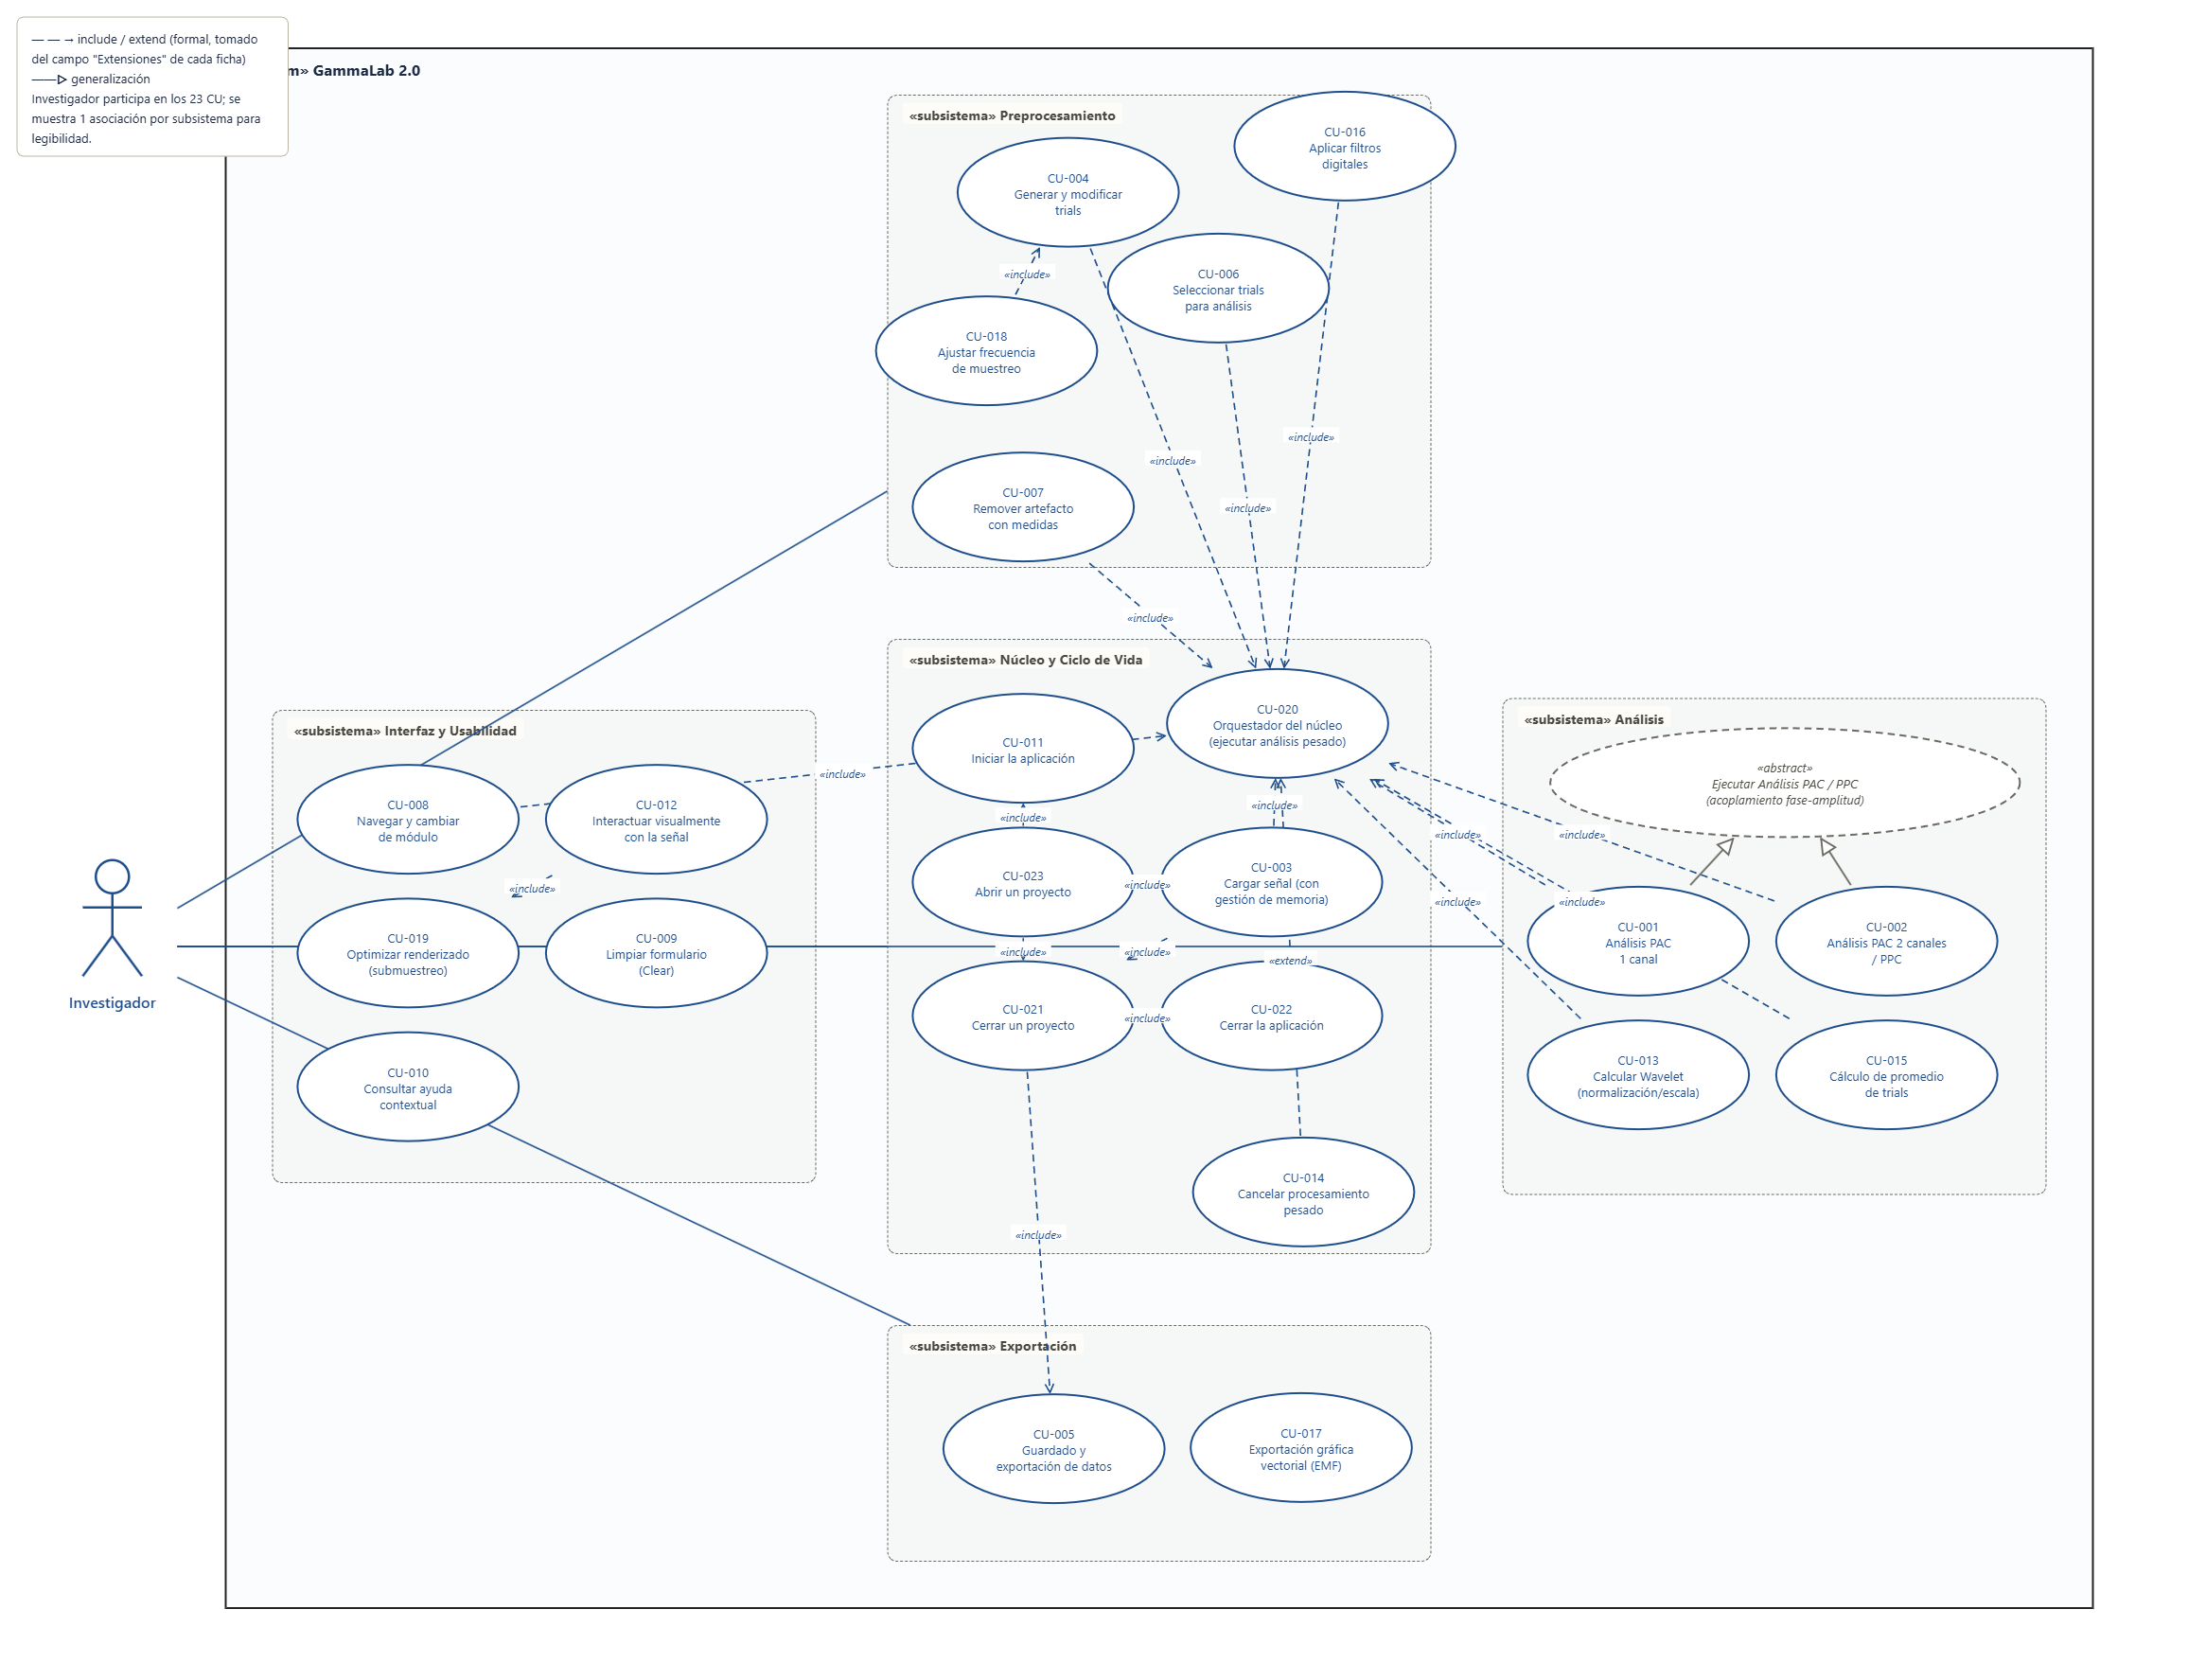
\includegraphics[width=\textwidth]{diagrama_casos_de_uso}
  \caption{Diagrama de casos de uso del sistema Gamma Lab 2.0}
  \label{fig:diagrama-casos-uso}
\end{figure}

Esta correspondencia entre subsistemas y componentes se detalla a continuación:

\begin{itemize}
    \item \textbf{Subsistema de Núcleo y Ciclo de Vida.} Agrupa los casos de uso que gestionan el estado global de la aplicación; inicio, apertura y cierre de proyectos, carga de señal con gestión de memoria y cierre de la aplicación— junto con el orquestador del núcleo, encargado de despachar todo cómputo pesado y de habilitar su cancelación. Los casos de uso de Preprocesamiento y Análisis que implican cómputo intensivo se apoyan en este subsistema mediante relaciones de inclusión.

    \item \textbf{Subsistema de Interfaz y Usabilidad.} Agrupa los casos de uso que gobiernan la navegación entre módulos, la interacción visual con la señal (zoom, lectura de coordenadas, butterfly), el renderizado fluido de señales pesadas mediante submuestreo, la limpieza de formularios y la ayuda contextual.

    \item \textbf{Subsistema de Preprocesamiento.} Agrupa los casos de uso que transforman la señal antes de cualquier análisis: la generación y modificación de trials, la selección de los trials que participan en un cálculo, la remoción de artefactos de estimulación con medidas de referencia previas al cambio, el ajuste de la frecuencia de muestreo y la aplicación de filtros digitales.

    \item \textbf{Subsistema de Análisis.} Agrupa las técnicas de procesamiento que constituyen el propósito analítico de la herramienta: el cálculo de la transformada Wavelet, el promedio de trials, y el análisis de acoplamiento fase-amplitud en su variante intra-canal (un canal) e inter-canal (dos canales y coherencia de fase, PPC), estas dos últimas modeladas como especializaciones de un caso de uso abstracto que comparte el procedimiento de cálculo.

    \item \textbf{Subsistema de Exportación.} Agrupa el guardado y exportación de datos del proyecto y la exportación gráfica en formato vectorial de los resultados analíticos.
\end{itemize}


\subsection{Restricciones}

Esta sección define los límites técnicos, normativos y operativos que condicionan el diseño, la implementación y el despliegue de Gamma Lab 2.0.

\subsubsection{Restricciones Generales}

El sistema opera íntegramente en inglés, tanto en la interfaz como en los mensajes de error y las alertas; ante fallos internos o errores del usuario, estos mensajes deben ser claros y no interrumpir el flujo de ejecución en curso. Asimismo, debe soportar la carga de archivos con múltiples canales y permitir ejecutar análisis sobre al menos uno de ellos, habilitando la selección de dos canales cuando el análisis sea de tipo inter-canal. Las gráficas, tablas y resultados numéricos que se generen deben poder exportarse desde la misma interfaz.

\subsubsection{Restricciones de Software}

El sistema mantiene una arquitectura modular orientada a plugins, en la que el Kernel orquesta la ejecución y permite incorporar nuevas capacidades sin modificar los plugins existentes. Se desarrolla en Python 3.11--3.12 y se distribuye como aplicación ejecutable localmente en Windows, aunque también puede ejecutarse directamente desde el código fuente del repositorio oficial.

El procesamiento de señales se apoya en NumPy, SciPy, MNE, TensorPAC y PyWavelets, mientras que la interfaz gráfica se construye con PySide6 y los componentes Qt; los formatos de entrada soportados son \texttt{.abf}, \texttt{.edf}, \texttt{.bdf} y \texttt{.mat}. La paralelización del Kernel, por su parte, se implementa mediante los mecanismos de hilos y \textit{multiprocessing} incluidos en la biblioteca estándar de Python.

\subsubsection{Restricciones de Hardware}

El sistema debe ejecutarse en Windows 10 de 64 bits o superior, sobre un equipo que cumpla con los siguientes requerimientos mínimos:

\begin{itemize}
    \item CPU de 4 núcleos a 2.0 GHz.
    \item 8 GB de RAM.
    \item 1 GB de VRAM.
    \item 3 GB de almacenamiento libre.
\end{itemize}


%=====================================================================
\capitulo{DISEÑO DE LA SOLUCIÓN}

\subsection{Arquitectura}
\pendiente

\subsection{Vistas de arquitectura}
\pendiente

\subsubsection{Vista lógica}
\pendiente

\subsubsection{Vista física}
\pendiente

\subsubsection{Vista de procesos}
\pendiente

\subsection{Diseño detallado}
\pendiente

\subsubsection{Estructura del sistema}
\pendiente

\subsubsection{Comportamiento del sistema}
\pendiente

\subsection{Tecnologías}
\pendiente

%=====================================================================
\capitulo{DESARROLLO DE LA SOLUCIÓN}

\subsection{Implementación}
\pendiente

\subsection{Producto}
\pendiente

\subsubsection{Funcionalidad 1}
\pendiente

\subsubsection{Funcionalidad 2}
\pendiente

\subsubsection{Funcionalidad 3}
\pendiente

%=====================================================================
\capitulo{PRUEBAS DE DESARROLLO}

\subsection{Metodología aplicada}
\pendiente

\subsection{Entorno y herramientas}
\pendiente

\subsection{Organización y documentación}
\pendiente

%=====================================================================
\capitulo{RESULTADOS}

\subsection{Resumen de pruebas unitarias}
\pendiente

\subsection{Observaciones y hallazgos}
\pendiente

\subsection{Resumen de pruebas comparativas contra el sistema de referencia}
\pendiente

\subsection{Observaciones y hallazgos}
\pendiente

\subsection{Resumen de pruebas de aceptación del usuario}
\pendiente

\subsection{Observaciones y hallazgos}
\pendiente

%=====================================================================
\capitulo{CONCLUSIONES}

\subsection{Análisis de Impacto del Proyecto}
\pendiente

\subsubsection{A corto, mediano y largo plazo}
\pendiente

\subsubsection{Impacto en Ingeniería de Sistemas}
\pendiente

\subsubsection{Impacto en Contextos Globales, Económicos, Ambientales y Sociales}
\pendiente

\subsection{Conclusiones y Trabajo Futuro}
\pendiente

\subsubsection{Conclusiones}
\pendiente

\subsubsection{Trabajo futuro}
\pendiente

%=====================================================================
\capitulo{REFERENCIAS}

\begin{thebibliography}{9}

\bibitem{singh2023}
A. K. Singh y S. Krishnan, ``Trends in EEG signal feature extraction applications,'' \textit{Frontiers in Artificial Intelligence}, vol. 5, art. 1072801, ene. 2023, doi: 10.3389/frai.2022.1072801. [En línea]. Disponible: \url{https://pmc.ncbi.nlm.nih.gov/articles/PMC9905640/}.

\bibitem{walla2025}
P. Walla, ``The Power of Time: Editorial on the Advantages of Electroencephalography (EEG) and Event-Related Potentials (ERPs) in Affective and Cognitive Neuroscience,'' \textit{Brain Sciences}, vol. 15, n.\textsuperscript{o} 10, art. 1054, sep. 2025, issn: 2076-3425, doi: 10.3390/brainsci15101054. [En línea]. Disponible: \url{https://www.mdpi.com/2076-3425/15/10/1054}.

\bibitem{srinivasan2025}
K. Jayalaksshme Srinivasan, P. Periasamy, y S. Gunasekaran, ``Motor Imagery and Motor Execution: A Narrative Review of Electroencephalographic (EEG) Signatures, Methodological Consistency, and Translational Applications,'' \textit{Cureus}, vol. 17, n.\textsuperscript{o} 9, art. e93011, sep. 2025, doi: 10.7759/cureus.93011. [En línea]. Disponible: \url{https://pmc.ncbi.nlm.nih.gov/articles/PMC12550537/}.

\bibitem{chaddad2023}
A. Chaddad, Y. Wu, R. Kateb, y A. Bouridane, ``Electroencephalography Signal Processing: A Comprehensive Review and Analysis of Methods and Techniques,'' \textit{Sensors}, vol. 23, n.\textsuperscript{o} 14, art. 6434, ene. 2023, issn: 1424-8220, doi: 10.3390/s23146434. [En línea]. Disponible: \url{https://www.mdpi.com/1424-8220/23/14/6434} (Visitado: 28-04-2026).

\bibitem{vanes2025}
M. W. J. van Es, C. Gohil, A. J. Quinn, y M. W. Woolrich, ``osl-ephys: a Python toolbox for the analysis of electrophysiology data,'' \textit{Frontiers in Neuroscience}, vol. 19, art. 1522675, feb. 2025, doi: 10.3389/fnins.2025.1522675. [En línea]. Disponible: \url{https://www.frontiersin.org/journals/neuroscience/articles/10.3389/fnins.2025.1522675/full}.

\bibitem{asencio2025}
S. Asencio Rodríguez, M. F. González Valencia, J. E. Martínez Clavijo, y G. V. Villalobos Rocha, ``Gamma Lab,'' Memoria de trabajo de grado, Programa de Ingeniería de Sistemas, Facultad de Ingeniería, Pontificia Universidad Javeriana, Bogotá, D.C., Colombia, nov. 2025.

\bibitem{gauthier2023}
C. Gauthier-Umaña, M. Valderrama, A. Múnera, y M. O. Nava-Mesa, ``BOARD-FTD-PACC: a graphical user interface for the synaptic and cross-frequency analysis derived from neural signals,'' \textit{Brain Informatics}, vol. 10, art. 12, may. 2023, issn: 2198-4026, doi: 10.1186/s40708-023-00191-x. [En línea]. Disponible: \url{https://link.springer.com/article/10.1186/s40708-023-00191-x}.

\end{thebibliography}

%=====================================================================
\capitulo{ANEXOS}

\subsection{MRCU - Matriz de Requerimientos y Casos de Uso}
\pendiente

\subsection{PMP — Project Management Plan}
\pendiente

\subsection{SAD - Software Architecture Document}
\pendiente

\subsection{SDD - Software Design Document}
\pendiente

\subsection{SRS - Software Requirements Specifications}
\pendiente

\subsection{TD - Test Document}
\pendiente

\subsection{MU - Manual de Usuario}
\pendiente

\subsection{VFP - Versión Final Propuesta de Proyecto}
\pendiente

\subsection{Aplicación de escritorio}
\pendiente

\end{document}
